%% Adaptado de 
%% http://www.ctan.org/tex-archive/macros/latex/contrib/IEEEtran/
%% Traduzido para o congresso de IC da USP
%%*****************************************************************************
% Não modificar

\documentclass[twoside,conference,a4paper]{IEEEtran}

%******************************************************************************
% Não modificar
\usepackage{IEEEtsup} % Definições complementares e modificações.
\usepackage[utf8]{inputenc} % Disponibiliza acentos.
\usepackage[T1]{fontenc}
\usepackage[english,brazil]{babel}
%% Disponibiliza Inglês e Português do Brasil.
\usepackage{latexsym,amsfonts,amssymb} % Disponibiliza fontes adicionais.
\usepackage{theorem} 
\usepackage[cmex10]{amsmath} % Pacote matemático básico 
\usepackage{url} 
%\usepackage[portuges,brazil,english]{\usepackage{soul,color}babel}
\usepackage{graphicx}
\usepackage{amsmath}
\usepackage{amssymb}
\usepackage{color}
\usepackage[pagebackref=true,breaklinks=true,colorlinks,bookmarks=false]{hyperref}
\usepackage[tight,footnotesize]{subfigure} 
\usepackage[noadjust]{cite} % Disponibiliza melhorias em citações.
\usepackage{soulutf8,color} % Highlight
%%*****************************************************************************

\begin{document}
\selectlanguage{brazil}
\renewcommand{\IEEEkeywordsname}{Palavras-chave}

%%*****************************************************************************

\urlstyle{tt}
% Indicar o nome do autor e o curso/nível (grad-mestrado-doutorado-especial)
\title{Inferência fuzzy aplicada à prevenção de colisão com o robô NAO}
\author{%
 \IEEEauthorblockN{André Pinheiro Borba\,\IEEEauthorrefmark{1} \\
 				   Giuliano Roberto Pinheiro\,\IEEEauthorrefmark{2} \\
                   Rodrigo Elizeu Gonçalves\,\IEEEauthorrefmark{3}}
 \IEEEauthorblockA{\IEEEauthorrefmark{1}%
                   Ciência da Computação - Graduação/PIF \\
                   E-mail: andrepibo@gmail.com \\
                   \IEEEauthorrefmark{2}%
                   Ciência da Computação - Aluno Especial \\
                   E-mail: giulianorp2010@gmail.com \\
                   \IEEEauthorrefmark{3}%
                   Ciência da Computação - Aluno Especial \\
                   E-mail: rodrigoegoncalves@gmail.com}
}

%%*****************************************************************************

\maketitle

%%*****************************************************************************
% Resumo do trabalho
\begin{abstract}
Este projeto trata do problema de locomoção com prevenção a impactos, com outros objetos, de robôs do tipo NAO. Desenvolvemos um sistema de inferência fuzzy para controlar a locomoção destes robôs, baseado na leitura de seus sonares, em cenários diversos. O desenvolvimento do projeto foi amparado por simuladores e bibliotecas de terceiros. O projeto foi desenvolvido utilizando Python, NAOqi e o simulador Webots. Ao final do projeto obtivemos um sistema fuzzy que direcionava a locomoção do robô e sua velocidade, prevenindo colisões. Ao longo deste relatório apresentamos formalmente o problema e discorremos à respeito da solução desenvolvida.

\end{abstract}

% Indique três palavras-chave que descrevem o trabalho
\begin{IEEEkeywords}
NAO, inferência fuzzy, colisão
\end{IEEEkeywords}

%%*****************************************************************************
% Modifique as seções de acordo com o seu projeto


\section{Introdução}

Atualmente a robótica está presente em diversos segmentos, do militar ao entretenimento. No segmento de uso geral, um robô em especial tem se destacado nos últimos anos. O NAO é um robô humanóide, capaz de andar, cantar e dançar. De origem francesa, é considerado como um dos mais avançados robôs da atualidade. Apesar dos seus 57 cm de altura, o NAO é equipado com câmeras, sensores táteis, de pressão, sonares e diversos outros.

Em cenários diversos, fazer com que um robô se locomova com inteligência é um desafio. Neste trabalho buscamos desenvolver um modelo fuzzy que manipule a locomoção de um robô NAO com base em dados obtidos através de seus sensores.

Este relatório primeiro descreve uma definição formal do problema em questão, em seguida elabora sucintamente em como o trabalho proposto foi desenvolvido. O relatório prossegue abordando os métodos utilizados, relata e discute os resultados e é sumarizado em uma conclusão.


\section{Definição do problema}

\subsection{Estado inicial}
O agente está localizado em uma posição inicial $(x_i, y_i)$, em uma das extremidades de um corredor (entre duas paredes laterais), direcionado para a posição final $(x_f, y_f)$ (extremidade oposta).

\subsection{Problema}
Fazer o agente se locomover através do corredor até alcançar a posição final, sem que ocorram colisões com as paredes.

\subsection{Ambiente}
\begin{LaTeXdescription}
\item[Parcialmente observável:] o agente não sabe a configuração completa do ambiente, apenas à sua distância para as paredes.
\item[Determinístico:] o próximo estado depende apenas do movimento feito pelo agente no estado atual.
\item[Estático:] não há mudanças no ambiente.
\item[Contínuo:] os sensores e atuadores utilizam medidas contínuas.
\item[Agente único:] apenas o robô NAO.
\item[Sequencial:] a sequência de ações do agente tem efeitos no longo prazo (sua posição).
\item[Desconhecido:] os sensores utilizados pelo agente não permitem que ele tenha conhecimento do estado completo do ambiente.
\item[Tipo do agente:] foram utilizados dois agentes, um puramente reativo e outro reativo retroalimentado, que considera decisões anteriores.
\end{LaTeXdescription}


\section{Trabalho proposto}

Este projeto consiste de uma implementação de um sistema fuzzy para o problema anteriormente descrito. O sistema será reponsável por definir as ações do robô, isto é, para qual direção o mesmo deve se locomover a cada instante de forma a alcançar o objetivo e satisfazer as restrições do problema. 

Para a realização deste trabalho foi-se utilizado o simulador de robótica Webots\textsuperscript{\textregistered}, que simula a interação do robô com cenários que representam o ambiente. O simulador possui uma interface gráfica que permite visualizar o ambiente e as ações do agente.  A abordagem utilizada pelos autores para modelar o problema são descritos na seção IV, enquanto os resultados são discutidos na seção V.


\section{Materiais e métodos}
Está seção irá tratar dos materiais e métodos utilizados para o desenvolvimento do projeto. Será descrito inicialmente o robô utilizado e suas principais características. Na sequência, caracterizamos o ambiente virtual utilizado para simular as ações do robô e apresentamos os cenários utilizados para os experimentos. Em seguida, o modelo fuzzy é apresentado seguido das especificações de implementação e ambiente de desenvolvimento.

\subsection{Robô}
O NAO é um robô humanóide, com 57 cm de altura e equipado com diversos sensores e atuadores. Suas versões mais novas possuem 26 graus de liberdade, o que faz dele um robô extremamente versátil, como é representado na figura~\ref{fig:fig1}. 

\begin{figure}[ht]
\centering
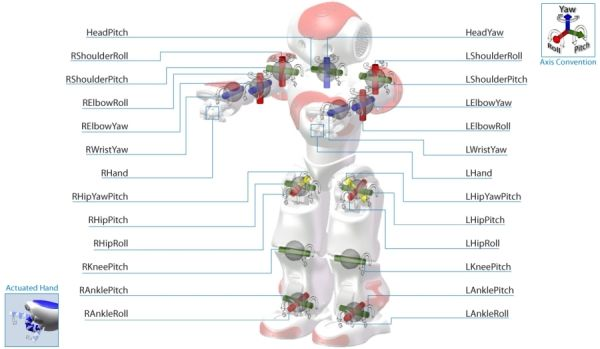
\includegraphics[width=1\hsize]{figuras/nao1.jpg}
\caption{Robô NAO.}
\label{fig:fig1}
\end{figure}

No que diz respeito a software, suas funcionalidades são executas por um sistema operacional baseado em linux. O principal software para controle do NAO é o NAOqi, responsável por controlar toda e qualquer recurso e operação fornecidos pelo robô. 

Para programar o robô utiliza-se uma interface provida pela Aldebaran, que estabelece uma conexão com o robô através de uma interface de rede e faz requisições e recebe respostas. É uma arquitetura cliente-servidor na qual o robô opera como servidor. Requisições podem transmitir comandos que irão controlar as ações do robô, ou recuperar dados capturados pelos sensores. A figura~\ref{fig:fig2} descreve como o NAOqi interage com as funcionalidades primitivas do robô.

\begin{figure}[ht]
\centering
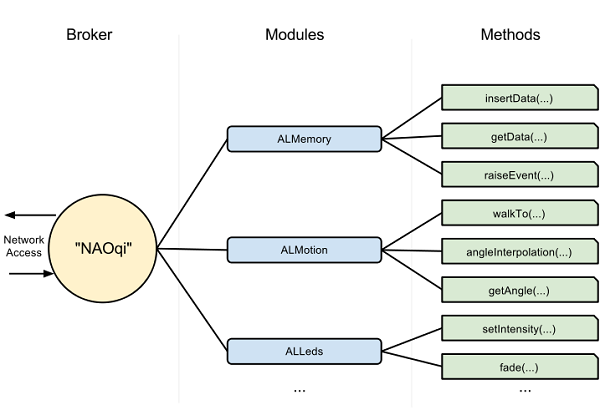
\includegraphics[width=1\hsize]{figuras/naoqi.jpg}
\caption{Interação do NAOqi com as funções primitivas do robô.}
\label{fig:fig2}
\end{figure}

O NAO é equipado com sonares localizados na parte frontal de seu torso, um par de receptor e transmissor de cada lado, ver figura~\ref{fig:fig3}. Seu funcionamento é simples, os transmissores emitem ondas sonoras supersônicas que são refletidas quando colidem com alguma superficie e são detectadas pelos receptores. O tempo de ida e volta das ondas determina a distância entre o NAO e a superfície, ver figura~\ref{fig:fig4}. Seus sonares possuem uma frequência de 40kHz e um raio de detecção que varia entre $[0.25;2.55]$ m ~\cite{AldebaranNaoSonars}. 

Neste projeto, os sonares fornecem dados que são utilizados como entrada para o sistema fuzzy. A cada instante a distância entre o robô e as paredes laterais do corredor são utilizadas para determinar a próxima ação.

\begin{figure}[ht]
\centering
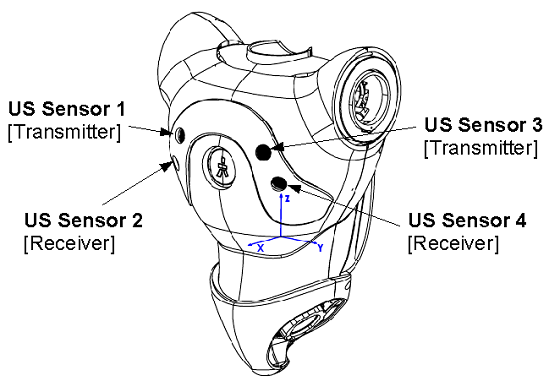
\includegraphics[width=1\hsize]{figuras/nao-sonar1.jpg}
\caption{Sonares do NAO.}
\label{fig:fig3}
\end{figure}

\begin{figure}[ht]
\centering
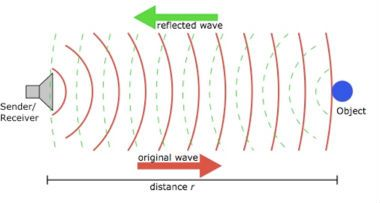
\includegraphics[width=1\hsize]{figuras/nao-sonar2.jpg}
\caption{Funcionamento do sonar.}
\label{fig:fig4}
\end{figure}

\begin{figure}[ht]
\centering
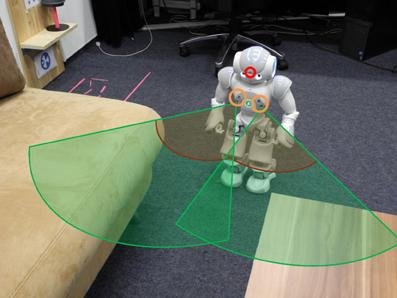
\includegraphics[width=1\hsize]{figuras/nao-sonar3.jpg}
\caption{Sonares do NAO em ação.}
\label{fig:fig5}
\end{figure}

\subsection{Ambiente virtual}
As simulações do projeto foram realizadas no simulador Webots\textsuperscript{\textregistered}. Este simulador provê um grande leque de recursos para o projeto de variados tipos ambientes e configurações de robôs. As propriedades de cada objeto, tais como forma, cor, textura e massa são configuráveis pelo usuário. Uma grande gama de sensores e atuadores estão disponíveis para equipar cada robô.

Nós preparamos diversos cenários diferentes para testar os modelos criados, cada qual com um nível de dificuldade diferente. Neste contexto, ser mais difícil significa que o cenário oferece mais obstáculos para que o robô se locomova sem colisões, como por exemplo curvas e espaço de movimentação restrito. As figuras~\ref{fig:fig6} e~\ref{fig:fig7} apresentam um cenário fácil e difícil respectivamente.

\begin{figure}[ht]
\centering
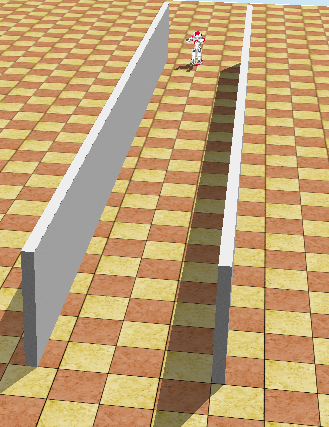
\includegraphics[width=1\hsize]{figuras/corredor-facil-2.png}
\caption{Cenário fácil.}
\label{fig:fig6}
\end{figure}

\begin{figure}[ht]
\centering
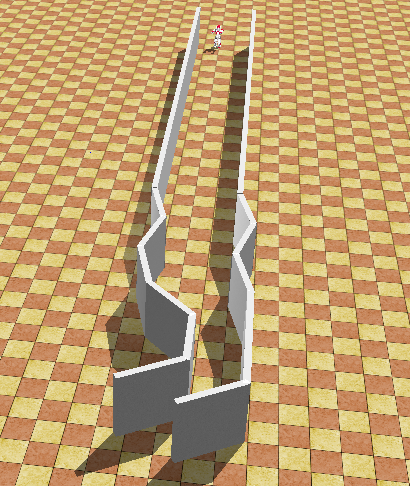
\includegraphics[width=1\hsize]{figuras/corredor-dificil-2.png}
\caption{Cenário difícil.}
\label{fig:fig7}
\end{figure}

Tivemos alguns problemas com os sonares do modelo do NAO disponibilizado pelo Webots\textsuperscript{\textregistered}. Apesar de o protótipo ser anunciado como tendo a configuração dos sonares similar à de fábrica com abertura e formato de cone com 60º, não conseguimos utilizá-lo com esses valores, pois ele não estava conseguindo identificar as distâncias das paredes, identificando somente objetos a sua frente, então modificamos para um abertura já um pouco maior que a que seria padrão, de aproximadamente 120º (2,09 radianos).

Outra alteração que fizemos do modelo do NAO foi para ele se aproximar mais do real, modificando a quantidade de raios dos sensores de 6 para 10 (exemplo na Figura~\ref{fig:fig8}).
A configuração para utilizar o NAO modificado está descrita na seção configuração de ambiente~\ref{sec:ambiente}.

\begin{figure}[ht]
\centering
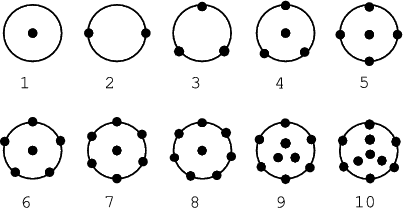
\includegraphics[width=1\hsize]{figuras/ray_orbits.png}
\caption{Exemplos possíveis configurações do sonar.}
\label{fig:fig8}
\end{figure}

\subsection{Modelo}
\subsubsection*{Agente Reativo}
O primeiro modelo proposto foi o mais simples possível, pois foi utilizado como base para as evoluções, até chegar-se a versão melhorada descrita após essa. Esse modelo utiliza como entrada os sonares da esquerda e da direita.

As variáveis de entrada são fuzzyficadas de acordo com as figura \ref{fig:sonar-fuzzy0}, usando funções triangulares.

\begin{figure}[ht]
\centering
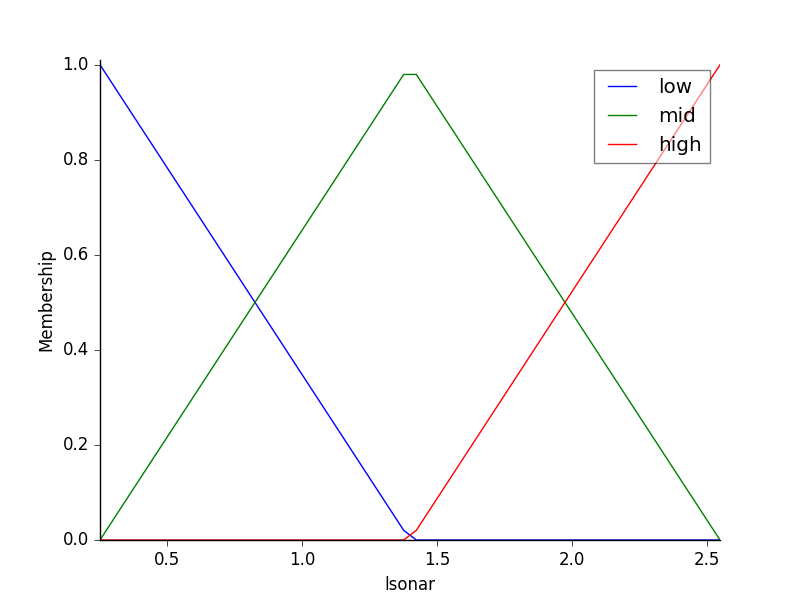
\includegraphics[width=1\hsize]{figuras/sonar_fuzzy0.png}
\caption{Funções de fuzzyficação das entradas de sonar.}
\label{fig:sonar-fuzzy0}
\end{figure}

\begin{figure}[ht]
\centering
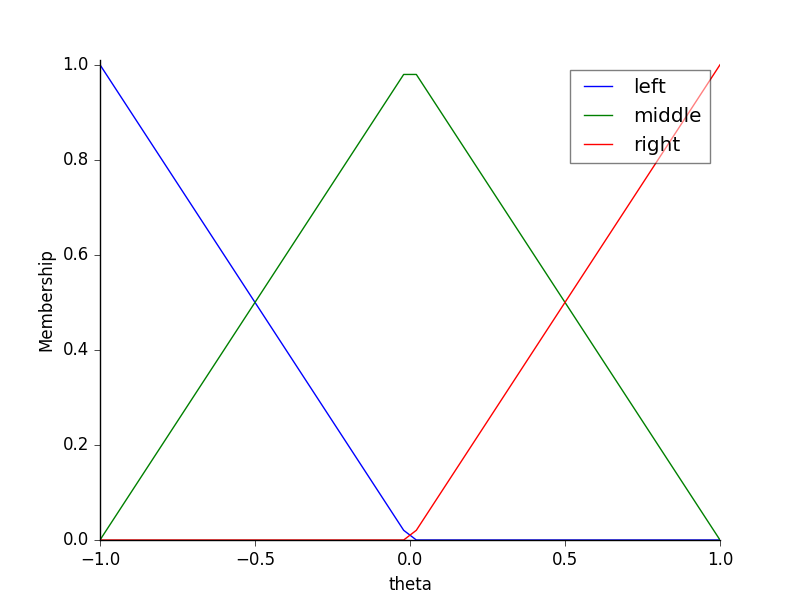
\includegraphics[width=1\hsize]{figuras/theta_fuzzy0.png}
\caption{Funções de fuzzyficação da entrada e saída de correção angular.}
\label{fig:theta-fuzzy0}
\end{figure}

Depois de defuzzyficado pelo método de centróide, a variável de saída theta é utilizada para definir a  correção do ângulo, dentro do intervalo real $[-1;1]$, sendo valores positivos os valores de giro no sentido anti-horário. A velocidade no eixo X é sempre contínua nesse modelo.

\subsubsection*{Agente Reativo Retroalimentado}
O segundo modelo proposto usa, além das duas entradas dos sonares da esquerda e da direita, um valor retroalimentado da última correção de trajetória executada pelo controlador fuzzy, que começa em zero no início da navegação.

As variáveis de entrada são fuzzyficadas de acordo com as figuras \ref{fig:sonar-fuzzy} e \ref{fig:theta-fuzzy}, usando funções triangulares, trapezoidais e gaussianas.

Na entrada dos sonares, as regiões cobertas pelas funções de pertinência ficam muito próximas do limite inferior de leitura dos sonares de forma a indicar situações onde o NAO não estaria apenas correndo perigo de choque, mas também de não conseguir entradas válidas para calcular os desvios necessários.

As variáveis de saída desse modelo são a correção angular e a velocidade do NAO no eixo $x$ com respeito a seu próprio referencial inercial\footnote{O NAO possui três possíveis referenciais inerciais: o seu próprio, calculado em relação à posição de seus pés, o referencial do torso, relativo à posição do corpo do robô, e o referencial do mundo, que corresponde à posição inicial do NAO quando ele sofre inicialização de movimento.}. Ambos os valores não tem unidade já que representam uma fração do máximo desempenho que o NAO consegue alcançar sem perder o equilíbrio. Os valores de correção de ângulo foram tratados dentro do intervalo real $[-1;1]$, sendo valores positivos os valores de giro no sentido anti-horário. Já os valores de velocidade estão no intervalo real $[0;1]$, portanto excluindo velocidades negativas que resultariam no movimento retrógrado do robô.

Uma vez fuzzificadas, as entradas prosseguem pelo sistema de controle que usa regras estabelecidas por algumas observações triviais sobre movimentação como: aplicar correções com menor velocidade quando as leituras indicarem proximidade demasiada dos obstáculos, continuar em linha reta mesmo que as leituras de distância comecem a diminuir, já que pode ocorrer de o movimento de correção não ser necessário, e aplicar correções sem diminuir a velocidade de caminhada caso haja espaço suficiente para realizar a manobra. Pequenos ajustes que cuidam de casos específicos foram adicionados empiricamente para controlar alguns casos mais extremos.

\begin{figure}[ht]
\centering
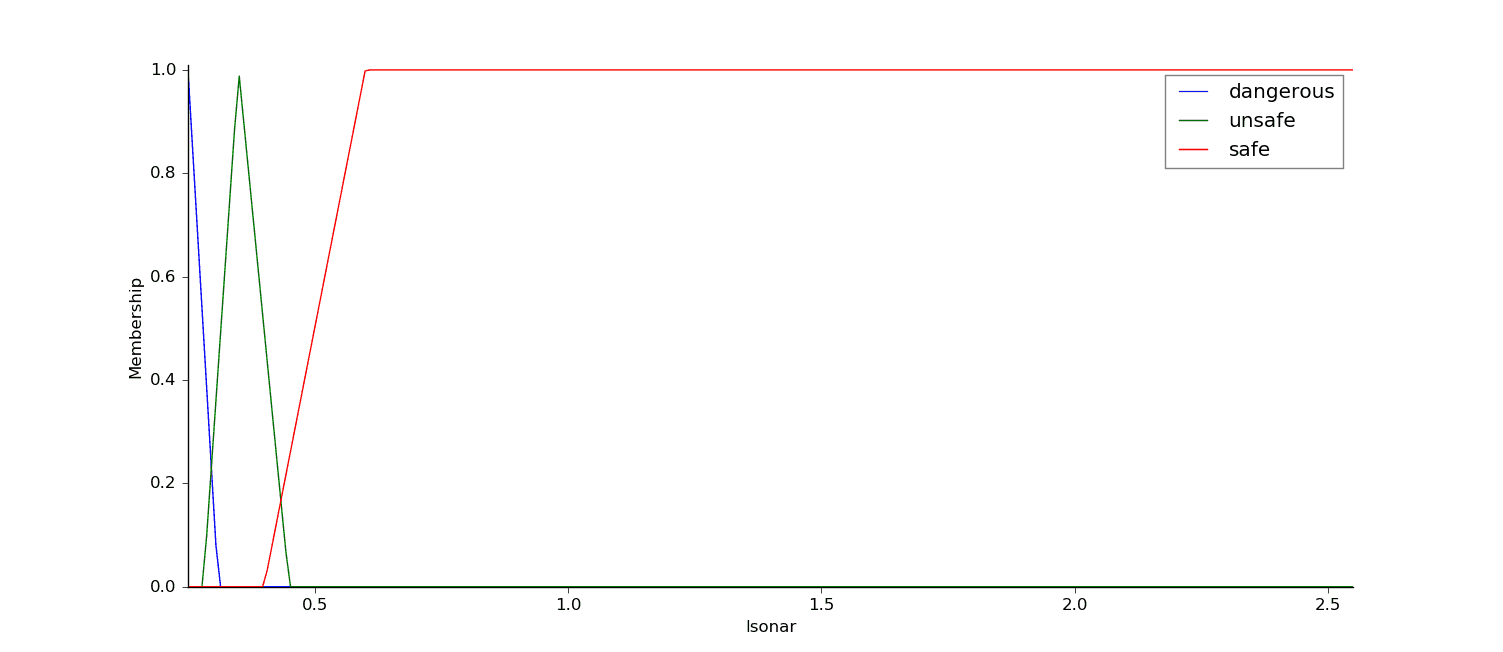
\includegraphics[width=1\hsize]{figuras/sonar_fuzzy.png}
\caption{Funções de fuzzyficação das entradas de sonar.}
\label{fig:sonar-fuzzy}
\end{figure}

\begin{figure}[ht]
\centering
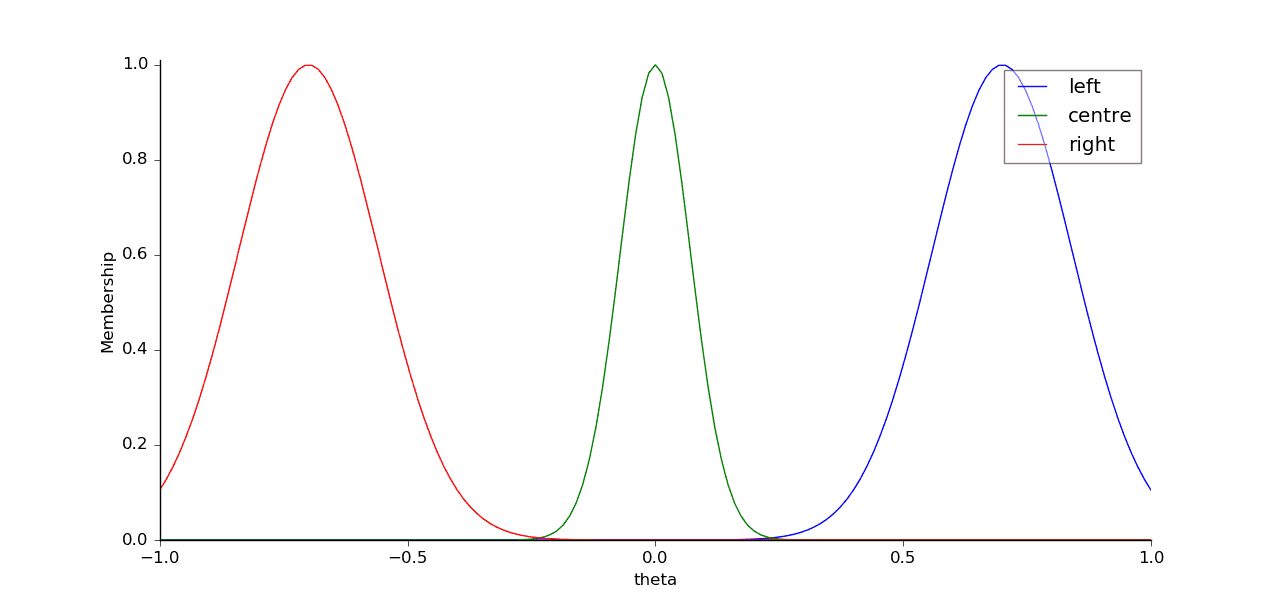
\includegraphics[width=1\hsize]{figuras/theta_fuzzy.png}
\caption{Funções de fuzzyficação da entrada e saída de correção angular.}
\label{fig:theta-fuzzy}
\end{figure}

\begin{figure}[ht]
\centering
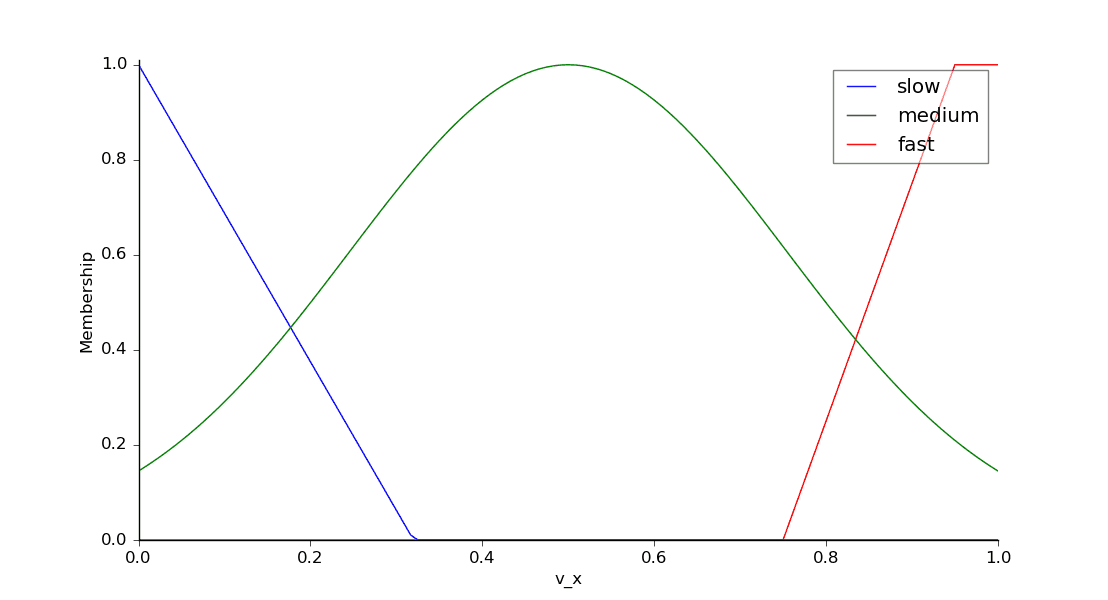
\includegraphics[width=1\hsize]{figuras/velocity_fuzzy.png}
\caption{Funções de fuzzyficação da saída de velocidade no eixo $x$.}
\label{fig:velocity-fuzzy}
\end{figure}

Uma vez interpretadas as regras, as variáveis consequentes são calculadas pelo controlador e desfuzzificadas pelo método do centroide.

Fora do sistema de inferência, essas variáveis de ajuste são recebidas pelo \textit{loop} de controle, que atualiza os valores de navegação do NAO usando a velocidade obtida do sistema fuzzy e uma combinação convexa do ajuste obtido pelo sistema de inferência na iteração corrente, $\theta_i$, e o da iteração anterior, $\theta_{i-1}$. Nossos experimentos nos levaram à combinação $\theta_c$, descrita na equação \ref{eq:convex}.

\begin{align}
	\theta_c = 0.3 \theta_{i-1} + 0.7 \theta_i
\label{eq:convex}
\end{align}

Essa combinação permitiu uma mudança um pouco mais amena do robô quando colocado diante de ambientes um pouco mais estreitos, criando uma espécie de ``efeito de memória'' na correção angular, daí vindo o nome do parâmetro resultante dessa escolha: \textit{memory factor}.

O loop principal então atualiza o valor da última correção efetuando $\theta_{i-1} \leftarrow \theta_i$ e bloqueia o avanço do loop por meio segundo, tempo suficiente para o NAO executar algum movimento antes de sofrer a próxima atualização.

Após um certo tempo de navegação, a condição de parada (tempo limite) é atingida, forçando o robô a parar e entrar em modo de descanso para indicar o final do script de controle.

Não foi implementada função objetivo com base em pontos no mapa ou distância percorrida. Nossa implementação tentou ser independente de restrições dadas por esse tipo de métrica. Embora fosse de interesse que esse tipo de medida de desempenho fosse incluída nos experimentos, resolvemos estressar o modelo usando corredores curvos e, muitas vezes, estreitos além dos limites inferiores de capacidade dos sonares como \textit{tradeoff}.

\subsection{Ambiente}
\label{sec:ambiente}
Todos os experimentos deste projeto foram executados em ambiente Linux (Ubuntu 14.10). 
A versão do simulador foi o Webots\textsuperscript{\textregistered} PRO 8.2.1 e a biblioteca do NAO foi o Aldebaran Python SDK 2.1.4. O próximo tópico descreve em detalhes as demais bibliotecas Python utilizadas para a implementação do projeto.

O procedimento para executar uma simulação do nosso projeto é composto de 6 partes:

\begin{enumerate}
\item Instalar as bibliotecas necessárias.
\item Editar as variáveis de PATH nos scripts setup\_naoqi.sh e env\_run.sh para os diretórios de instalação das bibliotecas.
\item Substituir o NAO.proto do Webots\textsuperscript{\textregistered} pelo modelo disponibilizado no código fonte do projeto~\cite{AnnaPawlicka2013}~\cite{CyberboticsNao}  (na versão utilizada do Linux, o arquivo fica localizado em ~/.local/share/Cyberbotics/Webots/8.2/projects/robots/\\
aldebaran/protos/Nao.proto)
\item Iniciar o Webots\textsuperscript{\textregistered} e carregar o cenário de teste que se deseja simular.
\item Executar o script setup\_naoqi.sh
\item Executar o script env\_run.sh. É facultativo passar um script Python como argumento. No caso deste projeto, utilizar \textit{./env\_run.sh naovigate[x].py} como argumento para controlar as ações do robô.
\end{enumerate}

\subsection{Implementação}
Este projeto foi desenvolvido em Python pois é uma linguagem flexível e poderosa que possibilita desenvolver protótipos e ideias rapidamente. Além disso, há um SDK Python oficial para programar o NAO. 

Os autores fizeram uso de diversas bibliotecas públicas para a implementação deste modelo, em especial a biblioteca Skfuzzy para desenvolver o modelo.  A implementação foi feita de forma incremental, ao longo do processo foram-se desenvolvidas diversas provas de conceito para verificar e validar as ideias e funcionalidades. Fizemos uso das bibliotecas matplotlib 1.5.1, numPy 1.11.1 e scikit\_fuzzy 0.2.


\section{Resultados e discussão}

\subsection{Diferentes abordagens para construção do modelo fuzzy}
Durante o desenvolvimento do projeto elaboramos dois modelos fuzzy diferentes. O primeiro foi uma abordagem com uma tendência minimalista onde as variáveis CRISP eram os valores dos sonares e a saída obtida seria simplesmente uma mudança na direção de caminhada do robô. Apesar de funcionar bem em cenários fáceis (paredes paralelas), esta abordagem se mostrou insuficiente em cenários mais complexos, que contavam com a presença de quinas e curvas.

O segundo modelo, apresentado na seção IV, possui uma complexidade maior e considera o resultado da iteração anterior como entrada para a geração atual. Tal modelo manipula na direção e velocidade do robô, o que aumenta sua eficiência em cenários mais desafiadores, com curvas mais fechadas.

\subsection{Limitações}
No decorrer do desenvolvimento deste projeto detectamos algumas limitações no que diz respeito ao uso do sonar como sensor para guiar a locomoção do robô e o uso de simulador para verificação dos resultados. Elencamos a seguir nossas principais conclusões a cerca desta matéria.

\begin{itemize}
\item O uso do sonar como sensor para guiar a locomoção do NAO se mostrou insuficiente. Isto ocorre por duas razões principais: 1) quando o ambiente ao redor do robô possui demasiadas variações de forma e ângulo (em relação à posição do robô) o sonar não é preciso o suficiente. 2) O simulador já calcula o resultado final dos raios do sonar e devolve somente um valor, não sendo possível utilizar outras formas de se calcular a distância dos objetos.
\item Em alguns casos o NAO não consegue diferenciar, através do uso do sonar, o que está ocorrendo. Por exemplo, quando ele está andando em um corredor que fica cada vez mais estreito ele "confunde" com estar andando na direção de uma parede. Isto ocorre por que os sonares esquerdo e direito detectam a mesma distância.
\item Inconsistência no uso do simulador. Em alguns momentos percebemos que o simulador reagia de formas diferentes ao mesmo comando, como por exemplo, executando o comando para ele andar em linha reta, com velocidade constante e sem nenhum obstáculo, o NAO mesmo assim as vezes tinha variações de velocidade, sendo que acontecia dele ficar dando passos sem sair do lugar por alguns momentos.
\end{itemize}

\subsection{Simulador}
Inicialmente, idealizamos utilizar o simulador V-REP\textsuperscript{\textregistered} para a realização deste projeto. Todavia, enfrentamos grande dificuldade em conseguir para configurá-lo e conseguir fazer o robô se locomover. Em dado momento foi possível fazê-lo, através da utilização de componentes de terceiros (Choreograph Suite\textsuperscript{\textregistered} e um adaptador que estabelecia uma conexão entre o Choreograph\textsuperscript{\textregistered} e o V-REP\textsuperscript{\textregistered}). Entretanto tal composição de bibliotecas e ferramentas proporcionava resultados inconsistentes e insatisfatórios no que diz respeito a locomoção do robô, que se comportava de maneira pseudo-aleatória e se mostrou incapaz de andar em linha reta. 

Em um segundo momento experimentamos o Webots\textsuperscript{\textregistered}, e obtivemos resultados mais consistentes e por isso ele foi adotado como simulador do projeto. Nesta configuração utilizamos apenas o Webots\textsuperscript{\textregistered} e o NAOqi SDK.


\section{Conclusão}

No decorrer deste projeto desenvolvemos um sistema de inferência fuzzy para um problema aparentemente simples. A fim de alcançar nossos objetivos precisamos integrar diversas ferramentas e bibliotecas diferentes, e fazê-las funcionarem em conjunto, de maneira holística. Este foi um grande desafio do ponto de vista técnico, frenquetemente lidamos com situações e problemas inéditos.

Pensamos que construir esta integração entre todas as partes foi algo positivo, que pode influenciar futuros projetos. Não obstante, tal integração não é livre falhas. Detectamos perda de precisão ao usar o simulador a qual não sabemos a exata causa mas acreditamos que pode estar relacionada à \textit{delays} na comunicação e o relógio interno da simulação.

Caso fôssemos desenvolver este projeto novamente com certeza adotaríamos uma abordagem mais quantitativa, com enfoque maior na coleta de dados. Tal abordagem possibilitaria a utilização de outra técnica de inteligência artificial para este problema, como por exemplos aprendizado de máquina para otimizar os parâmetros do sistema de inferência fuzzy.

Como trabalhos futuros, seria interessante explorar métodos de suavização de dados sensoriais, como filtros aplicados em uma sequência de leituras passadas a fim de evitar correções bruscas do controlador causadas por descontinuidades do próprio ambiente, como quinas e outros objetos no caminho.


%******************************************************************************
% Referências - Definidas no arquivo Relatorio.bib

\bibliographystyle{IEEEtran}
\nocite{*}
\bibliography{Relatorio}


%******************************************************************************

\end{document}